% Это основная команда, с которой начинается любой \LaTeX-файл. Она отвечает за тип документа, с которым связаны основные правил оформления текста.
\documentclass{article}

% Здесь идет преамбула документа, тут пишутся команды, которые настраивают LaTeX окружение, подключаете внешние пакеты, определяете свои команды и окружения. В данном случае я это делаю в отдельных файлах, а тут подключаю эти файлы.

% Здесь я подключаю разные стилевые пакеты. Например возможности набирать особые символы или возможность компилировать русский текст. Подробное описание внутри.
\usepackage{packages}

% Здесь я определяю разные окружения, например, теоремы, определения, замечания и так далее. У этих окружений разные стили оформления, кроме того, эти окружения могут быть нумерованными или нет. Все подробно объяснено внутри.
\usepackage{environments}

% Здесь я определяю разные команды, которых нет в LaTeX, но мне нужны, например, команда \tr для обозначения следа матрицы. Или я переопределяю LaTeX команды, которые работают не так, как мне хотелось бы. Типичный пример мнимая и вещественная часть комплексного числа \Im, \Re. В оригинале они выглядят не так, как мы привыкли. Кроме того, \Im еще используется и для обозначения образа линейного отображения. Подробнее описано внутри.
\usepackage{commands}

% Пакет для титульника проекта
\usepackage{titlepage}

% Здесь задаем параметры титульной страницы
\setUDK{192.168.1.1}
% Выбрать одно из двух
% \setToResearch
\setToProgram

\setTitle{3D-renderer с нуля}
\setStage{(промежуточный, этап 2)}
\setGroup{191}
%сюда можно воткнуть картинку подписи
\setStudentSgn{
\includegraphics[width=2cm]{kikos.png}}
\setStudent{К.В. Амеличев}
\setStudentDate{16.04.2021}
\setAdvisor{Дмитрий Витальевич Трушин}
\setAdvisorTitle{доцент, к.ф.-м.н.}
\setAdvisorAffiliation{ФКН НИУ ВШЭ}
\setAdvisorDate{}
\setGrade{}	
%сюда можно воткнуть картинку подписи
\setAdvisorSgn{}
\setYear{2021}


% С этого момента начинается текст документа
\begin{document}

% Эта команда создает титульную страницу
\makeTitlePage

% Здесь будет автоматически генерироваться содержание документа
\tableofcontents

% Данное окружение оформляет аннотацию: краткое описание текста выделенным абзацем после заголовка
\begin{abstract}
В рамках данной работы я разрабатываю библиотеку для языка программирования C++, занимающуюся отрисовкой объектов в трехмерном пространстве. После написания библиотеки планируется сделать тестовое приложение на ее основе.
\end{abstract}

\newpage

\section{Введение}

В рамках изучения тех или иных геометрических объектов возникает необходимость их графического отображения. Сложность в визуализации трехмерных объектов в том, что их нельзя изобразить на бумаге одним рисунком без потери информации. Настоящий трехмерный объект можно повертеть в руках и разглядеть со всех сторон, а вот рисунок на бумаге или экране может быть непонятен.

В рамках данной работы создается библиотека для языка программирования C++, которая визуализирует объекты в трехмерном пространстве, требуя от пользователя минимальных усилий. Данная библиотека будет полезна тем, кто обрабатывает достаточно сложные объекты, чтобы не отрисовывать их вручную, но при этом недостаточно сложные, чтобы потребовалось большое количество настроек.

Задачами данной работы является исследование существующих технологий и принципов в сфере 3д-графики, разработка интерфейса, реализация функционала, создание тестового приложения, последующее документирование и оформление в едином стиле библиотеки с открытым исходным кодом, а также описание теоретических знаний, которые были получены и применены в рамках исследования и разработки проекта.



\begin{center}\textbf{Весь исходный код проекта находится в репозитории по следующей \href{https://github.com/kik0s/3d-framework}{\color{blue}{ссылке}}} \end{center}

Также используются следующие источники информации:

\begin{enumerate}
\item \cite{vtkBook} --- сопроводительная инструкция к большому пакету для работы с 3d-графикой, в которой рассказываются основные принципы создания подобных приложений.
\item \cite{Math3d} --- математическая основа для библиотеки.
\item \cite{urtech}--- курс лекций по компьютерной графике
\end{enumerate}

\subsection{Функциональные требования}

\begin{itemize}
\item Отрисовка 3д-объектов.
\item База стандартных объектов для отрисовки, таких как куб или тетраедр.
\item Возможность создать любой триангулируемый объект в пространстве.
\item Задание параметров объекта, масштабирование, цвет.
\item Перемещение объектов.
\item Поворот объектов произвольным образом.
\item Возможность последовательной смены кадров, создание анимации
\item Обработка взаимодействия пользователя и приложения — пользовательские повороты и перемещения объектов, в частности по взаимодействию с клавиатурой
\item Возможность программно создавать и удалять объекты во время анимации.
\item Скрытие интерфейса отрисовки от пользователя — он отвечает только за создание объектов и операции с ними
\item Повороты и перемещение камеры
\item Возможность работы в статическом режиме — создать кадр и сохранить его как файл с изображением.
\end{itemize}

Интерфейс для пользователя следующий: у приложения один главный класс Application, представителя которого надо создать. После чего Application создает окно с графикой пользователя. Пользователь может добавлять объекты Application'у, давать ему команды для трансформации содержимого (перемещения, переворотов), а также в необходимый момент перерисовывать кадр.

\subsection{Технические требования}
\begin{itemize}
\item Разработка на языке C++
\item Сборка проекта с помощью CMake
\item Работа с 2д-графикой с помощью библиотеки SFML
\item Отрисовка графики на CPU
\item Открытый исходный код
\item Система поддержки версий Git
\item Ошибки программиста отлавливаются assert-ами
\item Системные ошибки обрабатываются как исключения и могут быть причиной аварийной остановки программы
\item Google C++ styleguide
\end{itemize}

Тестируется библиотека с помощью консольного приложения, в котором создаются произвольные 3d-объекты, после чего они переносятся на экран в интерактивном режиме, с возможностью перемещения, сдвигов и поворотов.

\newpage

\section{Изучение аналогов}

Поскольку в основном 3d-графика в программировании используется для создания игр, то почти все библиотеки, которые мне удалось найти, имели перегруженный интерфейс под игры, как у \href{http://polycode.org/features/}{\textcolor{blue}{Polycode}}, где надо создавать дополнительные xml-конфигурационные файлы.

Также есть такие популярные фреймворки, как OpenGL или Direct3d, но они настолько низкоуровневые, что при написании простого приложения почти все время уйдет на их изучение.

Получается, что у низкоуровневых библиотек нужно продумывать слишком много параметров, а у высокоуровневых библиотек сложная архитектура и протокол взаимодействия пользователя с библиотекой.

Разумеется, библиотека будет проигрывать в производительности аналогам, как минимум поскольку в ней не предусмотрена отрисовка через GPU. Но важной целью работы является именно создание архитектуры отрисовщика 3d-графики с нуля.

\newpage

\section{Содержательная часть}

\subsection{Основы 3d-графики}

При работе над 3d-рендерером достаточно важной частью работы является понимание математики, происходящей внутри обработчика графики. Основная проблема заключается в том, что на одни и те же объекты можно смотреть с разных сторон, и в зависимости от этого получать разную картинку. Поскольку все случаи не разберешь, на помощь приходит линейная алгебра.

\subsubsection{Объекты для отрисовки}

Все объекты разделяются на два типа~--- отрезки и треугольники. На самом деле, достаточно только треугольников, но отрезки рисовать значительно проще, при этом ими можно отображать каркасы объектов, что тоже имеет смысл.

Каждый объект задается набором отрезков и треугольников в глобальной системе координат. Отрезки можно использовать для отрисовки ребер фигуры, а поверхности можно триангулировать. Объекты, созданные из отрезков и треугольников, не меняют своего расположения в глобальной системе координат при передвижении камеры, а также могут двигаться независимо друг от друга. При этом в рамках одной фигуры все отрезки и треугольники находятся в относительной системе координат, где имеют свои относительные координаты. Если с объектом не происходит механических манипуляций, то в относительной системе координат координаты отрезков и треугольников будут неизменными.

\begin{center}
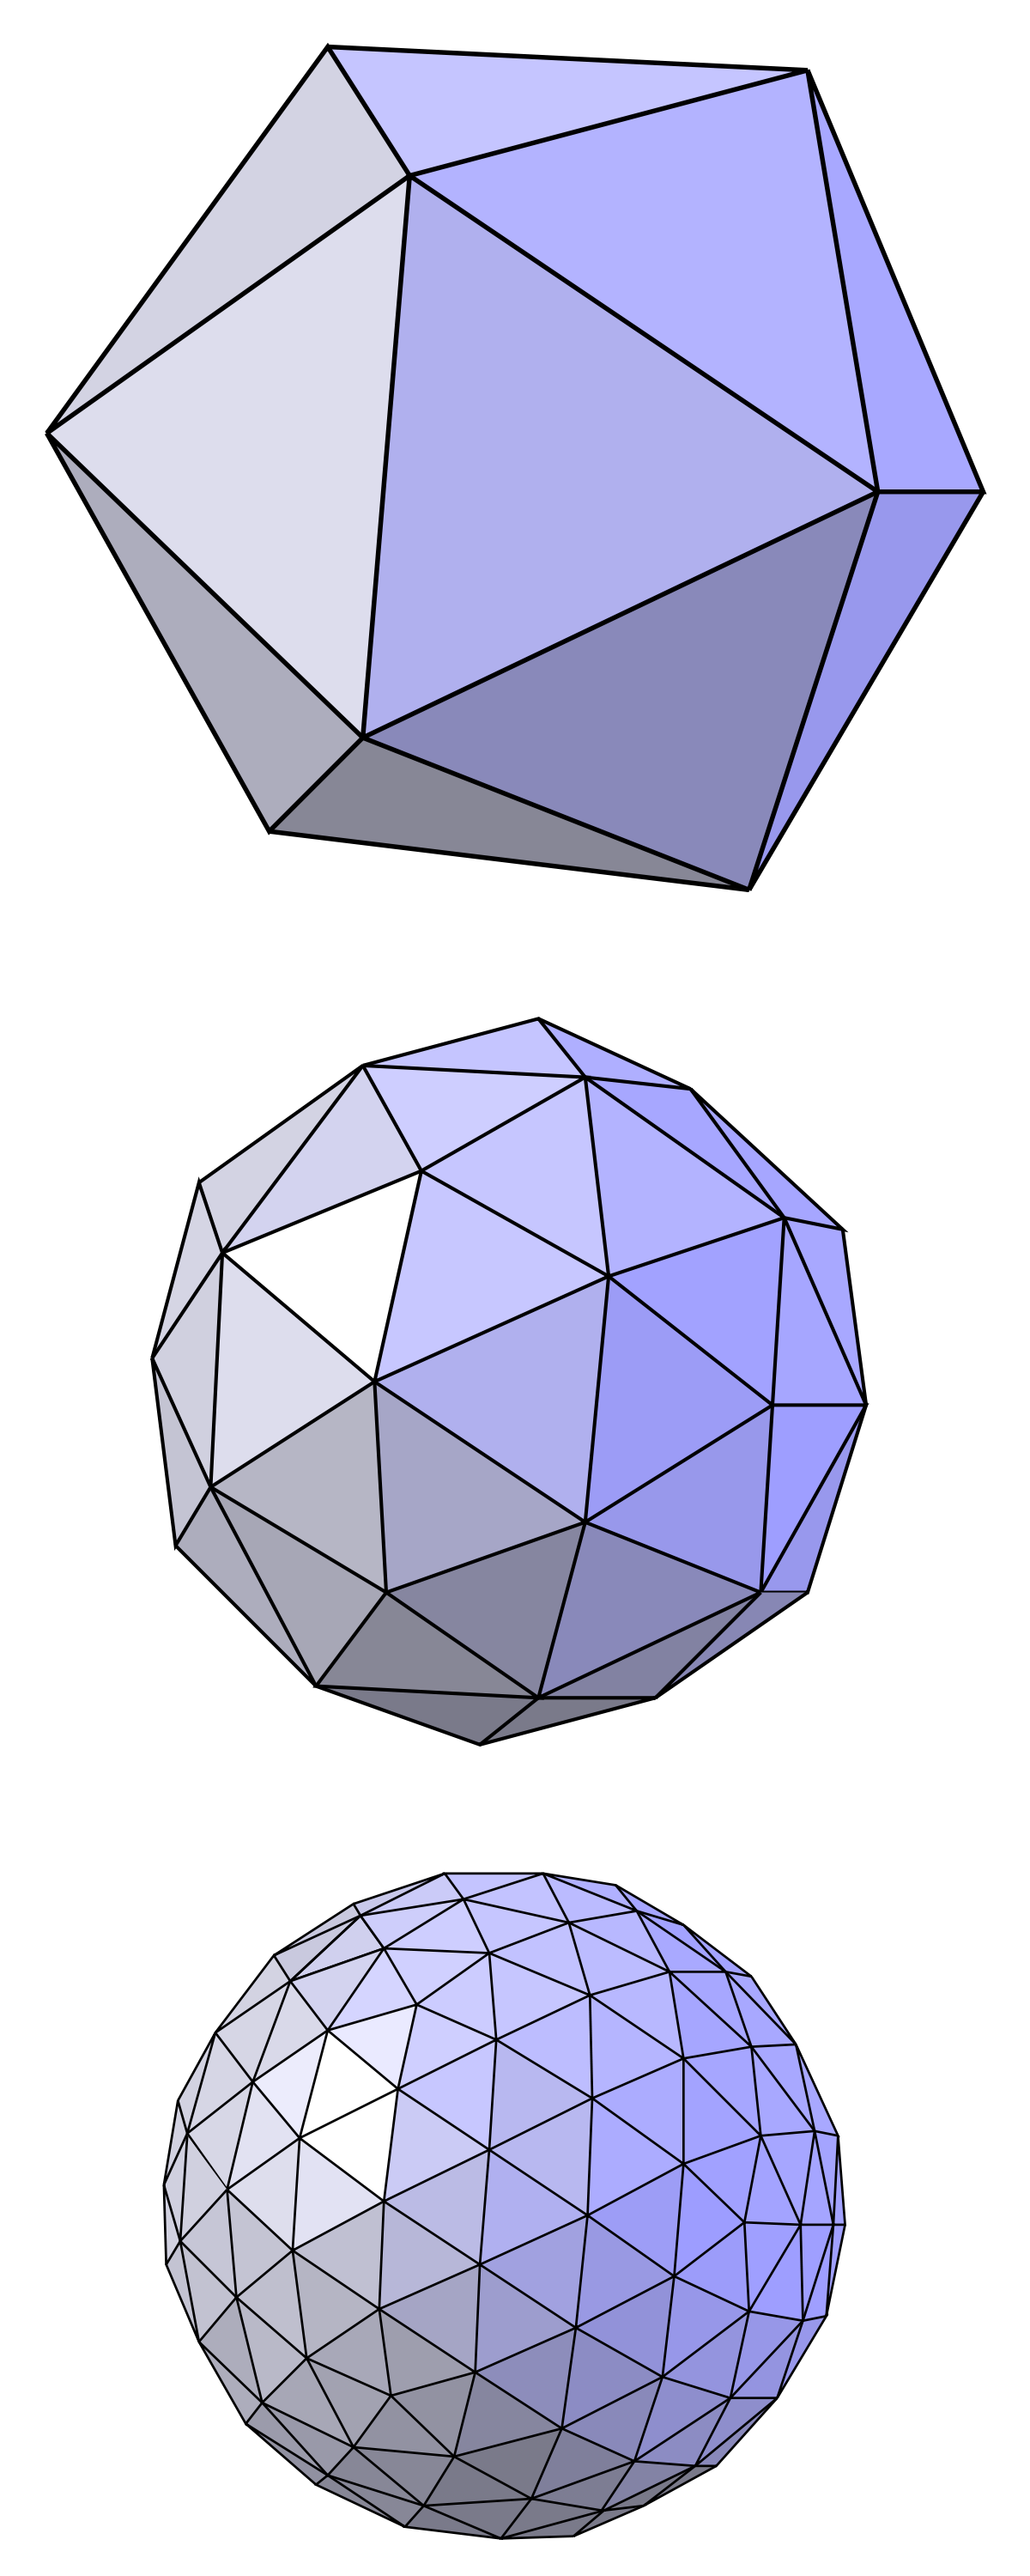
\includegraphics[width=4cm]{surfaces.png}
\end{center}

\subsubsection{Экран и камера}

\subsubsection{Общая последовательность шагов}

Объекты надо как-то отображать на экране. Экран представляется произвольной плоскостью в пространстве, на который проецируются все точки. Поскольку экран имеет ограниченный размер, то и на плоскости выбирается ограниченный прямоугольник. Те точки, которые попадут на прямоугольник экрана, и будут отрисованы. Остальные находятся вне поля зрения.

Для того, чтобы правильно выбирать прямоугольник экрана, используется объект камеры. Этот объект задается своим положением в пространстве ($O_c =  \begin{bmatrix} x_{camera} \\ y_{camera} \\ z_{camera} \end{bmatrix}$), а также системой из трех ортогональных векторов, которые = задают направление, в котором смотрит камера, а также координатную плоскость, параллельную плоскости экрана. Назовем направление камеры вектором $N_c$.

По направлению $N_c$ выбирается область видимости и прямоугольник экрана. Все вершины фигур проецируются на плоскость экрана через базисные векторы $A_c,\,B_c$. Каким образом проецируются? Для начала, вся система координат сдвигается на вектор $-N_c$. После этого берется матрица поворота для системы координат, которая приводит систему координат камеры к стандартной $oXYZ$. Иначе говоря, это такая матрица, котороя делает поворот мира, обратный к повороту камеры. $M \begin{bmatrix}A_c& B_c& N_c\end{bmatrix} = \begin{bmatrix} A & 0 & 0 \\ 0 & B & 0 \\ 0 & 0 & C \end{bmatrix}$.

Для того, чтобы добавить эффект перспективы, область видимости задается в виде усеченной четырехугольной пирамиды. Такой объект сложно спроецировать на экран, поэтому для начала его проективным преобразованием переводят в прямоугольный параллелипипед. После этого проекция оказывается просто отбрасыванием координаты.

У этого подхода есть еще одно приемущество. Отбрасываемая координата задает глубину точки относительно экрана. Поэтому, при прочих равных, надо будет в конкретном пикселе отрисовывать ту точку, которая имела меньшую глубину. Такой метод называется $z$-буфером.

\begin{center}
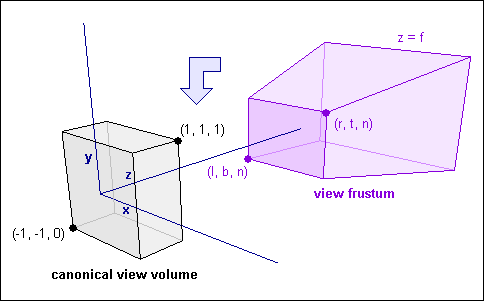
\includegraphics[width=6cm]{z-buffer.png}
\end{center}

Так что после поворота камеры происходит проективное преобразование, после чего искомый прямоугольник сначала масштабируется в куб $2 \times 2 \times 2$. У точки в кубе координаты $(x, y)$ проецируются на экран, а координата $z$ отвечает за глубину точки относительно экрана. 

\subsubsubsection{Однородные координаты}

Поскольку все операции с координатами имеет смысл выражать через векторы и матрицы, возникает проблема с тем, что не все афинные преобразования представляются произведением трехмерных матриц. Для этого вводят однородную систему координат, которая работает с четырехмерным пространством по следующему правилу:

$$\begin{pmatrix} x \\ y \\ z \end{pmatrix} \to \begin{pmatrix}x \\ y \\ z \\ 1\\ \end{pmatrix}$$

$$\begin{pmatrix}x \\ y \\ z \\ w\\ \end{pmatrix}, w \neq 0 \to \begin{pmatrix} \frac{x}{w} \\ \frac{y}{w} \\ \frac{z}{w}\end{pmatrix}$$

Такая система разрешает, во-первых, прибавить произвольное число к любой из координат трехмерного вектора:

$$\begin{bmatrix} 1 & 0 & 0 & a_x \\ 0 & 1 & 0 & a_y \\ 0 & 0 & 1 & a_z \\ 0 & 0 & 0 & 1\end{bmatrix} \cdot\begin{bmatrix} x \\ y \\ z \\ 1 \end{bmatrix} = \begin{bmatrix} x + a_x \\ y + a_y \\ z + a_z \\ 1 \end{bmatrix} \to \begin{bmatrix} x + a_x \\ y + a_y \\ z + a_z \end{bmatrix}$$

Также появляется возможноть разделить координаты на произвольную линейную функцию от координат:

$$\begin{bmatrix} 1 & 0 & 0 & 0 \\ 0 & 1 & 0 & 0 \\ 0 & 0 & 1 & 0 \\ k_x & k_y & k_z & 0\end{bmatrix} \cdot\begin{bmatrix} x \\ y \\ z \\ 1 \end{bmatrix} = \begin{bmatrix} x \\ y \\ z \\ k_xx + k_yy + k_zz\end{bmatrix} \to \begin{bmatrix}\frac{x}{k_xx + k_yy + k_zz} \\\frac{y}{k_xx + k_yy + k_zz} \\\frac{z}{k_xx + k_yy + k_zz} \end{bmatrix}$$

Утверждается, что такого дополнительного функционала хватает, чтобы сделать проективное преобразование пирамиды зрения в прямоугольный параллелепипед.


\subsubsubsection {Здоровенная матрица}
В итоге получается, что камера должна сделать большое преобразование из нескольких матриц:

\begin{enumerate}
	\item Сдвиг камеры в центр координат
	\item Поворот всего мира для перехода в базис камеры
	\item Проективное преобразование
	\item Сдвиг центра видимого параллелепипеда в центр координат
	\item Масштабирование в куб $2 \times 2 \times 2$
	\item Прообразование для получения пикселей экрана
\end{enumerate}

$$ M = \begin{bmatrix}\frac{Screen_x}{2} & 0 & 0 & \frac{Screen_x - 1}{2} \\ 
					  0 & \frac{Screen_y}{2} & 0 & \frac{Screen_y - 1}{2} \\
					  0 & 0 & 1 & 0 \\
					  0 & 0 & 0 & 1\end{bmatrix}\begin{bmatrix}
					  \frac{2}{r - l} & 0 & 0 & 0 \\ 
					  0 & \frac{2}{t - b} & 0 & 0 \\
					  0 & 0 & \frac{2}{n - f} & 0 \\
					  0 & 0 & 0 & 1\end{bmatrix}\begin{bmatrix}
					  1 & 0 & 0 & \frac{-l - r}{2} \\ 
					  0 & 1 & 0 & \frac{-b - t}{2} \\
					  0 & 0 & 1 & \frac{-n - f}{2} \\
					  0 & 0 & 0 & 1\end{bmatrix} \cdot $$$$\cdot \begin{bmatrix}
					  n & 0 & 0 & 0 \\
					  0 & n & 0 & 0 \\
					  0 & 0 & n + f & -nf \\
					  0 & 0 & n & 0
					  \end{bmatrix}\begin{bmatrix}
					  x_u & y_u & z_u & 0 \\
					  x_v & y_v & z_v & 0 \\
					  x_w & y_w & z_w & 0 \\
					  0 & 0 & 0 & 1
					  \end{bmatrix}\begin{bmatrix}
					  1 & 0 & 0 & -Camera_x \\
					  0 & 1 & 0 & -Camera_y \\
					  0 & 0 & 1 & -Camera_z \\
					  0 & 0 & 0 & 1
					  \end{bmatrix}$$



\begin{center}
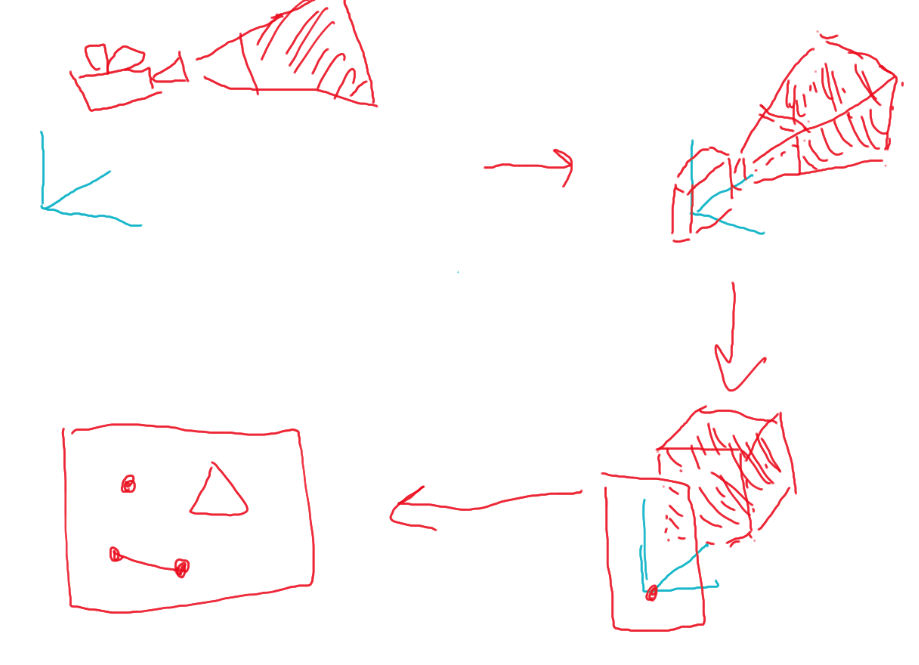
\includegraphics[width=6cm]{camera_pipeline.png}
\end{center}
\newpage
\subsection{Отрисовка двумерных объектов}
Дальше происходит отрисовка двумерных объектов на экране по пикселям и заданным вершинам. Для отрезка это достаточно несложная задача, а вот для заливки треугольника нужно придумывать эффективные способы. Автор использует так называемую <<сканирующую прямую>>~--- треугольник отрисовывается послойно, на каждом слое выделяется вертикальная полоса внутри треугольника, и заполняется только она.

Псевдокод отрисовки двумерного треугольника:

\begin{minted}{c++}
     for (int x = triangle2d.get_left_x(); x <= triangle2d.get_right_x(); x++) {
        // triangle logic to find the stripe
        min_y = find_min_y(triangle2d, x);
        max_y = find_max_y(triangle2d, x);

        double min_z = ...; // get z_value for 2d-point (x, min_y)
        double max_z = ...; // get z_value for 2d-point (x, max_y)
        for (int y = ceil(min_y); y <= floor(max_y); y++) {
        	// linear scaling for z
            z = (max_z - min_z) * (y - min_y) / (max_y - min_y);
            screen->set_pixel(x, y, z);
        }
    }
\end{minted}

Надо теперь понять, как найти min\_y, max\_y. Поиск min\_z, max\_z будет не очень сложным --- поскольку треугольник невырожденный, достаточно будет выделить в нем два базисных вектора, по ним выразить наш пиксель, затем с такими же коэффициентами взять базисные векторы треугольника в пространстве; полученную точку нужно будет преобразовать и найти ее z-value.

\begin{center}
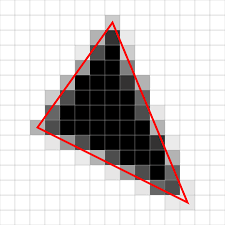
\includegraphics[width=10cm]{triangle.png}
\end{center}


\subsubsection{Сортировка точек в треугольнике}

Чтобы в треугольнике выделить полосу, нужно рассмотреть несколько случаев. Для того, чтобы уменьшить число случаев, имеет смысл заранее отсортировать все точки треугольника против часовой стрелки. Для этого нужно найти первую точку как самую левую (среди самых левых - самую нижнюю), после чего сравнить векторное произведение двух векторов $(B - A) \times (C - A)$.

Псевдокод:

\begin{minted}{c++}
Triangle2d::Triangle2d(sf::Vector2f _a, sf::Vector2f _b, sf::Vector2f _c): a(_a), b(_b), c(_c) {
    for (int i = 0; i < 3; i++) {
        order_[i] = i;
    }
    if (a.x > b.x || (a.x == b.x && a.y > b.y)) {
        std::swap(order_[0], order_[1]);
        std::swap(a, b);
    }
    if (a.x > c.x || (a.x == c.x && a.y > c.y)) {
        std::swap(a, c);
        std::swap(order_[0], order_[2]);
    }
    if (cross(b - a, c - a) < 0) {
        std::swap(order_[1], order_[2]);
        std::swap(b, c);
    }
}
\end{minted}

\subsubsection{Выделение полосы в треугольнике}

Чтобы для каждого слоя найти вертикальную полосу, я использую следующий алгоритм: точки треугольника заранее отсортированы против часовой стрелки, при этом первой в порядке сортировки идет самая левая, а среди самых левых --- самая нижняя. Дальше я реализую две симметричные функции для нахождения верхней и нижней границы полосы. Рассмотрим поиск нижней границы. Я смотрю на отрезок $AB$. Если он пересекает полосу, то точка находится на нем, ее можно выразить из линейного уравнения. Если он не пересекает полосу, то точка находится на соседнем отрезке $BC$, линейное уравнение решается для него. Мы добились такого расположения точек за счет предварительной сортировки.

Псевдокод поиска границы для полосы:

\begin{minted}{c++}
double find_min_y(triangle, x) {
    if (|triangle.b.x - x| < eps) {
        return triangle.b.y;
    }
    if (triangle.b.x > x) {
        v = triangle.a - triangle.b;
        if (|v.x < eps) {
            return triangle.a.y;   
        }
        k = (triangle.b.x - x) / v.x;
        v *= |k|;
        return (triangle.b + v).y;
    }
    else {
        v = triangle.c - triangle.b;
        if (|v.x| < eps) {
            return triangle.b.y;
        }
        k = (triangle.b.x - x) / v.x;
        v *= |k|;
        return (triangle.b + v).y;
    }
}

\end{minted}

\begin{center}
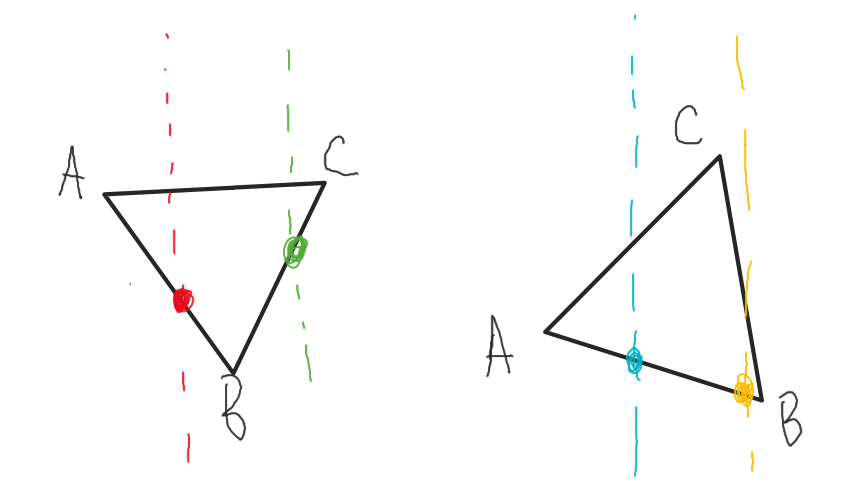
\includegraphics[width=9cm]{sweepline.png}
\end{center}


\subsubsection{Сложность}

Если оценить сложность, то мы выделим необходимую область за $O(w)$, где $w$~--- ширина треугольника. Таким образом, самая неэффективная часть в отрисовке треугольника~--- отрисовка каждого пикселя за $O(S_{\Delta})$. Но поскольку для любого растрового экрана это действие нам понадобится, можно считать, что алгоритм досточно эффективный для нашей задачи.


\newpage

\subsection{Библиотека: описание элементов}

\subsubsection{Авторское: Точки, матрицы, геометрия}

Матрицы Matrix нужны для работы с матричными вычислениями. Пользователю доступно создание матриц произвольного размера, операторы для сложения, вычитания и перемножения матриц. Также доступен поиск обратных матриц, выражение вектора через базис пространства, транспонирование.

Точки Point4d представляют собой набор из четырех координат или матрицу $4 \times 1$. Это объект, который нужен для удобной обертки над несколькими переменными. Для него также доступны арифметические операции, а также отождествление с вектором и возможность нахождения длины. Также есть отождествление 4d-точек с трехмерными через единичную последнюю координату (однородные координаты).

Для работы с двумерной геометрией используется класс двумерного треугольника Triangle2d. Основной его смысл — давать нужную информацию о треугольнике — координаты точек, сохраненные в отсортированном порядке.

Все многомерные треугольники для отрисовки передаются как объекты класса Triangle4d, который выступает в роли контейнера.

\subsubsection{Авторское: Объекты, мир}

Структура объектов такая: есть объекты типа WireObject, есть объекты типа SurfaceObject, являющиеся наследником типа WireObject. WireObject хранит каркас фигуры: точки и ребра, а SurfaceObject расширяет WireObject данными о триангулированной поверхности объекта. Взаимодействие пользователей происходит с объектами типа SurfaceObject. Мир World является просто контейнером, в котором лежат все объекты. Объекты можно\footnote{ когда-нибудь будет можно, строго говоря} поворачивать и двигать.

И объекты, и мир поддерживают возможность итерирования по своему содержимому: у объектов можно просмотреть все ребра и грани, а у мира можно посмотреть все объекты.

\subsubsection{Авторское: Камера}

Камера Camera отвечает за то, чтобы переводить объекты из системы координат мира в систему координат экрана. Для этого этот объект генерирует матрицу преобразования и применяет ее ко всем точкам, которые надо отобразить. Также камеру можно поворачивать и двигать, что отражается на матрице преобразования.

\subsubsection{Авторское: Экран}

Экран Screen нужен для растрового представления экрана. Он представляет собой несколько табличек с данными по каждому пикселю экрана с возможностью доступа и изменения. А именно, позволяет поставить значение цвета пикселя и узнать текущее значение $z$-буфера в точке.

\subsubsection{Авторское: Renderer}

Renderer отвечает за логику отрисовки. Он принимает набор объектов SurfaceObject, после чего берет отрезки и треугольники в многомерном пространстве, с помощью камеры Camera переносит их в двумерное пространство, выполняет алгоритм растеризации и переносит весь кадр на экран Screen, после чего отрисовывает кадр с помощью библиотеки SFML. 

\subsubsection{Авторское: Application}

Объект Application является основным объектом приложения для пользователя~--- именно оно осуществляет взаимодействие между всеми остальными объектами. Иначе говоря, Application берет все объекты SurfaceObject из контейнера World, после чего просит Renderer отрисовать эти объекты.

Также Application поддерживает интерактивный функционал, доступный в SFML ~--- позволяет пользователю настроить listener-ы на различные системные события, которые умеет отлавливать SFML (например, нажатие на клавиши).

\subsubsection{Стороннее: SFML}

\href{https://www.sfml-dev.org/}{\textcolor{blue}{SFML}} --- это библиотека для отрисовки 2d-графики. У нее есть два основных приемущества:

\begin{enumerate}

\item Достаточно простая.
\item Поддерживает создание интерактивных приложений.

\end{enumerate}

Используется для отрисовки массива точек (растеризованный экран), а также для отрисовки отрезков-ребер.


\newpage
\subsection{Библиотека: Pipeline}

\subsubsection{Описание.}

В итоге основной Pipeline получился таким:

\begin{itemize}

\item Application.update() вызовет Renderer.prepare(), чтобы очистить экран Screen.clear() и обновить матрицу преобразования Camera.create\_transform()
\item Application.update() вложенными циклами переберет сначала все объекты в мире, а потом все треугольники в объекте.
\item Эти треугольники отправятся на Renderer.draw() --- сначала Camera.project\_point() переведет их в координаты на экране, потом прогоняется алгоритм для двумерного треугольника: для каждой x-координаты находится полоса с помощью Triangle2d.find\_max\_y()/Triangle2d.find\_min\_y(). Чтобы узнать z-координату пикселя, надо узнать ее для двух крайних пикселей полосы; с помощью Matrix.solve\_system() двумерный вектор выражается по базису треугольника, после чего нужная z-величина получается взятием этих же векторов в 3-мерном пространстве с полученными коэффициентами\footnote{На самом деле можно без решения системы, потому что там всегда в одном из трех базисов координата будет скаляром вдоль ровно одного базисного вектора. Но поскольку там надо еще понять, вдоль какого вектора, то я пока что просто системку решаю.}
\item Полученные пиксели отправляются в Screen.draw(), где вычисляется ближайший пиксель к плоскости экрана (минимальная z-value)
\item Application.update() в самом конце делает Renderer.update(), который делает Screen.update(), который проходит по всем пикселям и вызывает Renderer.draw() для этого пикселя, в результате пиксель оказывается на экране.
\end{itemize}

\subsubsection{Схема.}

\begin{center}
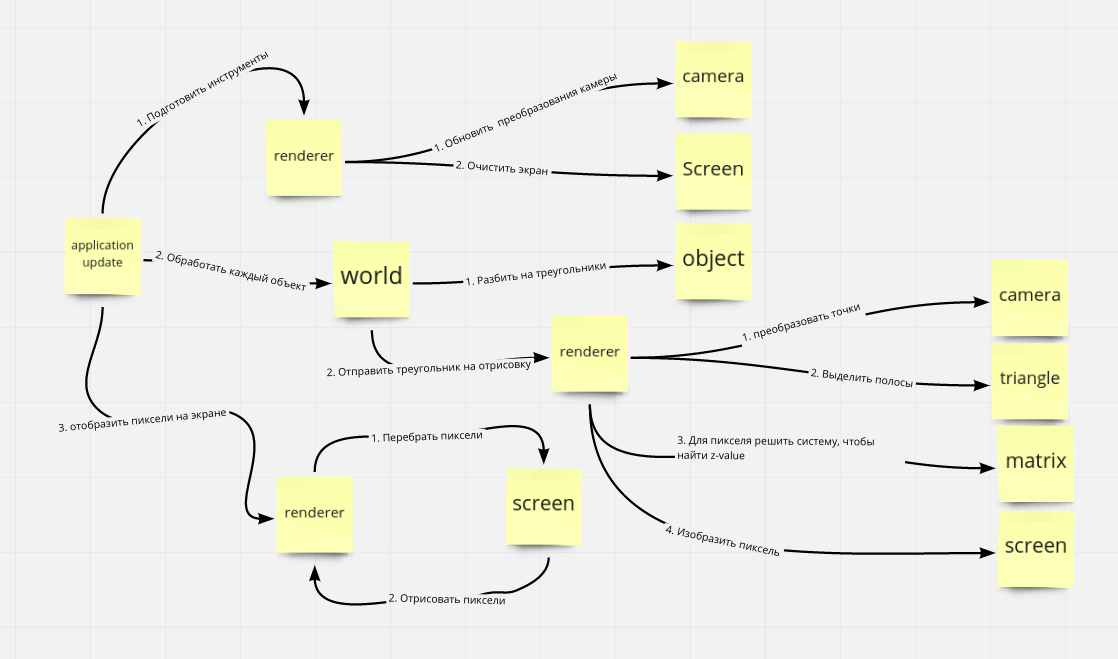
\includegraphics[width=15cm]{scheme_pipeline.png}
\end{center}


\subsubsection{Псевдокод,}

\begin{minted}{c++}
void Application::update() {
    renderer_->prepare();
    for (auto& object : *world_) {
        for (auto& triangle : object->triangles()) {
            renderer_->draw(triangle);
            triangles++;
        }
    }
    renderer_->update();
}

void Renderer::prepare() {
    window_.clear(sf::Color::White);
    screen_->clear();
    camera_->create_transform();
}

void Renderer::update() {
    screen_->update();
    window_.display();
}

void Renderer::draw(const Triangle4d& triangle4d) {
    
    Triangle2d triangle2d(camera_->project_point(triangle4d.a),
                          camera_->project_point(triangle4d.b),
                          camera_->project_point(triangle4d.c));
    
    sf::Vector2f left_point = triangle2d.get_left_point();
    sf::Vector2f right_point = triangle2d.get_right_point();
    
    Matrix<2, 2> basis = triangle2d.create_basis();
    for (int x = ceil(left_point.x); x <= floor(right_point.x); x++) {
        min_y = find_min_y(triangle2d, x);
        max_y = find_max_y(triangle2d, x);

        min_z = get_z(/* get z for (x, min_y) from basis and triangle2d and triangle4d */);
        max_z = get_z(/* get z for (x, max_y) from basis and triangle2d and triangle4d */);
        for (int y = ceil(min_y); y <= floor(max_y); y++) {
           	z = (max_z - min_z) * (y - min_y) / (max_y - min_y);
            screen_->set_pixel(x, y, z, sf::Color::Black);
        }
    }
}

void Camera::create_transform() {
    transform_ = canonical2Screen * rect2Canonical  *  move2Center *
    			* magic * transform_camera_.transpose() * move_camera;
}


Point4d Camera::transform_point(Point4d p) const {
    return transform_ * p;
}

sf::Vector2f Camera::project_point(Point4d p) const {
    Point4d transformed = transform_point(p);
    return {transformed.x / transformed.w, 
            transformed.y / transformed.w};
}

double Camera::get_z_value(Point4d p) const {
    return transform_point(p).z / transform_point(p).w;
}

void Screen::set_pixel(int x, int y, double z, sf::Color color) {
    if (x < 0 || y < 0 || x >= get_screen_size() || y >= get_screen_size() ||
        z > get_max_z_value() || z < get_min_z_value()) {
        return;
    }
    if (z < z_value_(x, y)) {
        z_value_(x, y) = z;
        color_(x, y) = color;
    }
}

void Screen::update() {
	vector<sf::Vertex> data;
    for (int i = 0; i < get_screen_size(); i++) {
        for (int j = 0; j < get_screen_size(); j++) {
            if (z_value_(i, j) < get_max_z_value()) {
                data.push_back(sf::Vertex(sf::Vector2f(i, j), color_(i, j)));
            }
        }
    }
    renderer_->draw(data);
}


\end{minted}

\newpage
\subsection{Тествое приложение и текущие результаты.}

Для теста на текущей стадии разработки используется приложение, в котором можно вращать и двигать кубик. Далее привожу две картинки того, как это у меня выглядит сейчас.

\begin{center}
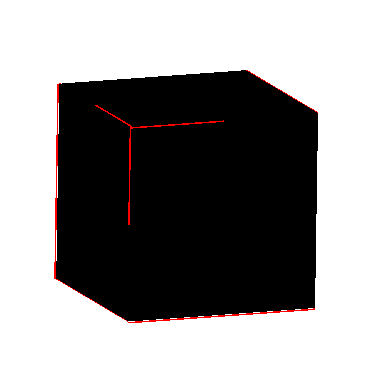
\includegraphics[width=5cm]{cube-1.png}

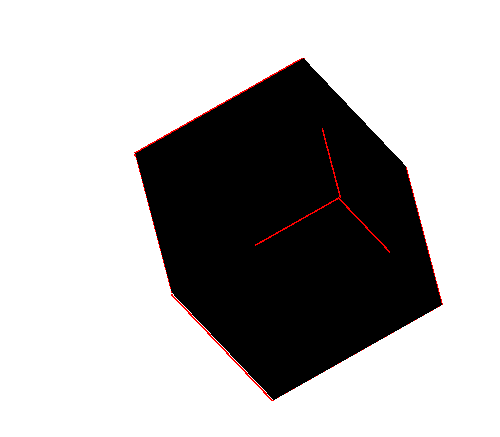
\includegraphics[width=5cm]{cube-2.png}
\end{center}




\bibliographystyle{plainurl}
\bibliography{bibl}

% Здесь текст документа заканчивается
\end{document}
% Начиная с этого момента весь текст LaTeX игнорирует, можете вставлять любую абракадабру.
